\chapter{Materiais e Métodos}\label{cap:ferramentas}

A ferramenta OpenCV \citeonline{itseez2015opencv} é uma biblioteca de código aberto focada em problemas de visão computacional em tempo real, desenvolvida pela intel e posteriormente pela Itseez, com suporte a múltiplas plataformas e uso gratuito sobre a licença de código aberto BSD. A ferramenta apresenta suporte a frameworks de aprendizado profundo, como TensorFlow, Pytorch e Caffe \citeonline{wiki:OpenCV} e contempla tanto funções básicas, para aplicações como processamento de imagem, alteração de cor ou resolução, até aplicações avançadas, como detecção facial, identificação de características e biometria.

Neste trabalho, será utilizada a função de detecção de faces da ferramenta opencv, que utiliza um classificador Haar em cascata baseado características, este é um método eficiente para reconhecimento de faces em imagens proposto por Paul Viola and Michael Jones, comunmente conhecido como método Viola-Jones, onde uma função é treinada com muitos exemplos positivos (imagens que contém o objeto a ser detectado) e negativos (imagens que não contém o objeto a ser detectado) e então utilizada para detectar as mesmas características em outras imagens. \cite{itseez2014theopencv}

\section{Algoritmo Viola-Jones}

O algoritmo Viola-Jones foi publicado em 2001, no paper "Rapid object detection using a boosted cascade of simple features" \citeonline{paper-viola-jones} e é famoso por sua capacidade de detecção de faces com muita velocidade, isso ocorre devido a 3 principais técnicas utilizadas: a imagem integral, o adaboost e o classificador em cascata.

A primeira etapa do algoritmo Viola-Jones consiste em tranformas a imagem original em uma imagem integral, isto é feito calculando o valor de cada pixel como a soma de todos os pixels que estão acima ou a esquerda do mesmo, como ilustrado na figura~\ref{fig:img-integral}.

\begin{figure}[htpb]
    \centering
    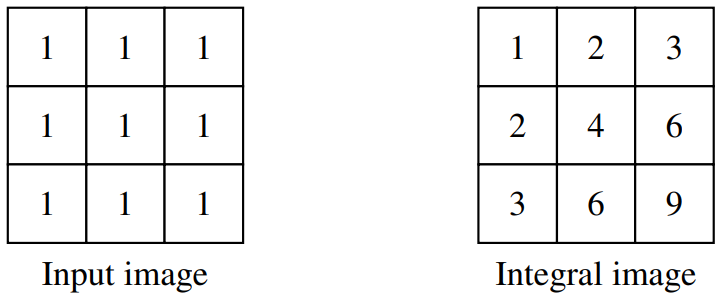
\includegraphics[scale=.3]{figs/imagem-integral.png}
    \caption{Imagem original (esquerda) e imagem integral (direita). Extraído de \citeonline{jensen2008implementingviolajones}}
    \label{fig:img-integral}
 \end{figure}

A utilização desta técnica permite calcular facilmente o tamanho de qualquer retângulo formado entre quatro pixels da imagem, conhecendo apenas o valor dos seus cantos, possibilitando assim a análise rápida de diversas partes da imagem. Tal calculo é feito definindo o retangulo a ser análisado e então aplicando o cálculo \ref{DEFINIR}.

\begin{figure}[htpb]
    \centering
    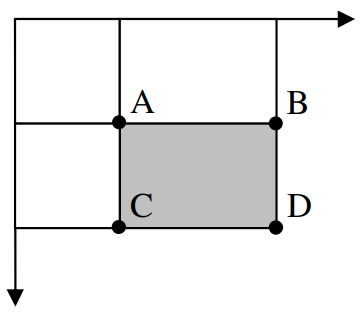
\includegraphics[scale=.3]{figs/imagem-integral-calculo.png}
    \caption{Representação da área da imagem a ser analisada. Extraído de \citeonline{jensen2008implementingviolajones}}
    \label{fig:img-integral}
 \end{figure}

 \begin{equation}\label{eq:img-integral}
    \text{ Soma do retângulo cinza } = D - (B + C) + A
\end{equation}


O classificador em cascata consiste na utilização de uma série de classificadores fracos, que combinados se tornam um classificador forte, mas estes são aplicados de forma sequencial, permitindo que imagens que certamente não possuem faces sejam rapidamente descartadas logo nas primeiras iterações, enquanto imagens com possíveis faces são classificadas por toda cascata, trazendo um elevado nível de confiança

https://pdfs.semanticscholar.org/40b1/0e330a5511a6a45f42c8b86da222504c717f.pdf
https://docs.opencv.org/4.1.0/d7/d8b/tutorial_py_face_detection.html

\section{Considerações Finais}

\lipsum[23]
